\subsection{观察者模式(Observer)}

\subsubsection{观察者模式简介}

观察者模式是一种软件设计模式,它用于实现一种一对多的依赖关系,使得每当一个对象的状态发生改变时,其他依赖于它的对象都能收到通知并自动更新。

观察者模式的一个常见应用场景是实现事件驱动的程序。例如,假设我们有一个用于表示按钮的类,它允许用户点击它,这样它就会触发一个事件。在这种情况下,我们可以使用观察者模式来处理这个事件,从而让其他对象能够监听这个事件并执行相应的操作。

例如,假设我们有一个按钮类,如下所示:

\begin{lstlisting}
class Button {
  constructor() {
    this.observers = [];
  }

  addObserver(observer) {
    this.observers.push(observer);
  }

  onClick() {
    // 触发事件
    for (const observer of this.observers) {
      observer.onClick();
    }
  }
}
\end{lstlisting}


这个类表示一个按钮,它包含一个用于保存观察者的数组和一个 addObserver 方法,用于向数组中添加新的观察者。当按钮被点击时,它会触发一个事件,并通知所有已注册的观察者。这样,观察者就能够监听按钮的点击事件,并执行相应的动作。

观察者模式具有以下优点:

\begin{enumerate}
\item 观察者模式可以实现一种松耦合的设计,使得观察者和被观察者之间不需要直接引用来进行通信。
\item 观察者模式可以提高系统的灵活性,因为它允许在不更改对象之间的关系的情况下添加新的观察者。
\item 观察者模式可以使得系统更加模块化,从而更容易实现和维护。
\end{enumerate}

\begin{enumerate}
\item 观察者模式可能会使得系统变得过于复杂,因为它需要维护被观察者和观察者之间的关系。
\item 观察者模式可能会导致性能问题,因为它需要在多个对象之间进行额外的通信。
\item 观察者模式可能会导致循环依赖,特别是在观察者和被观察者之间存在多对多的关系时。
\end{enumerate}

\subsubsection{观察者模式在项目中的应用}

\begin{figure}[h]
  \centering
  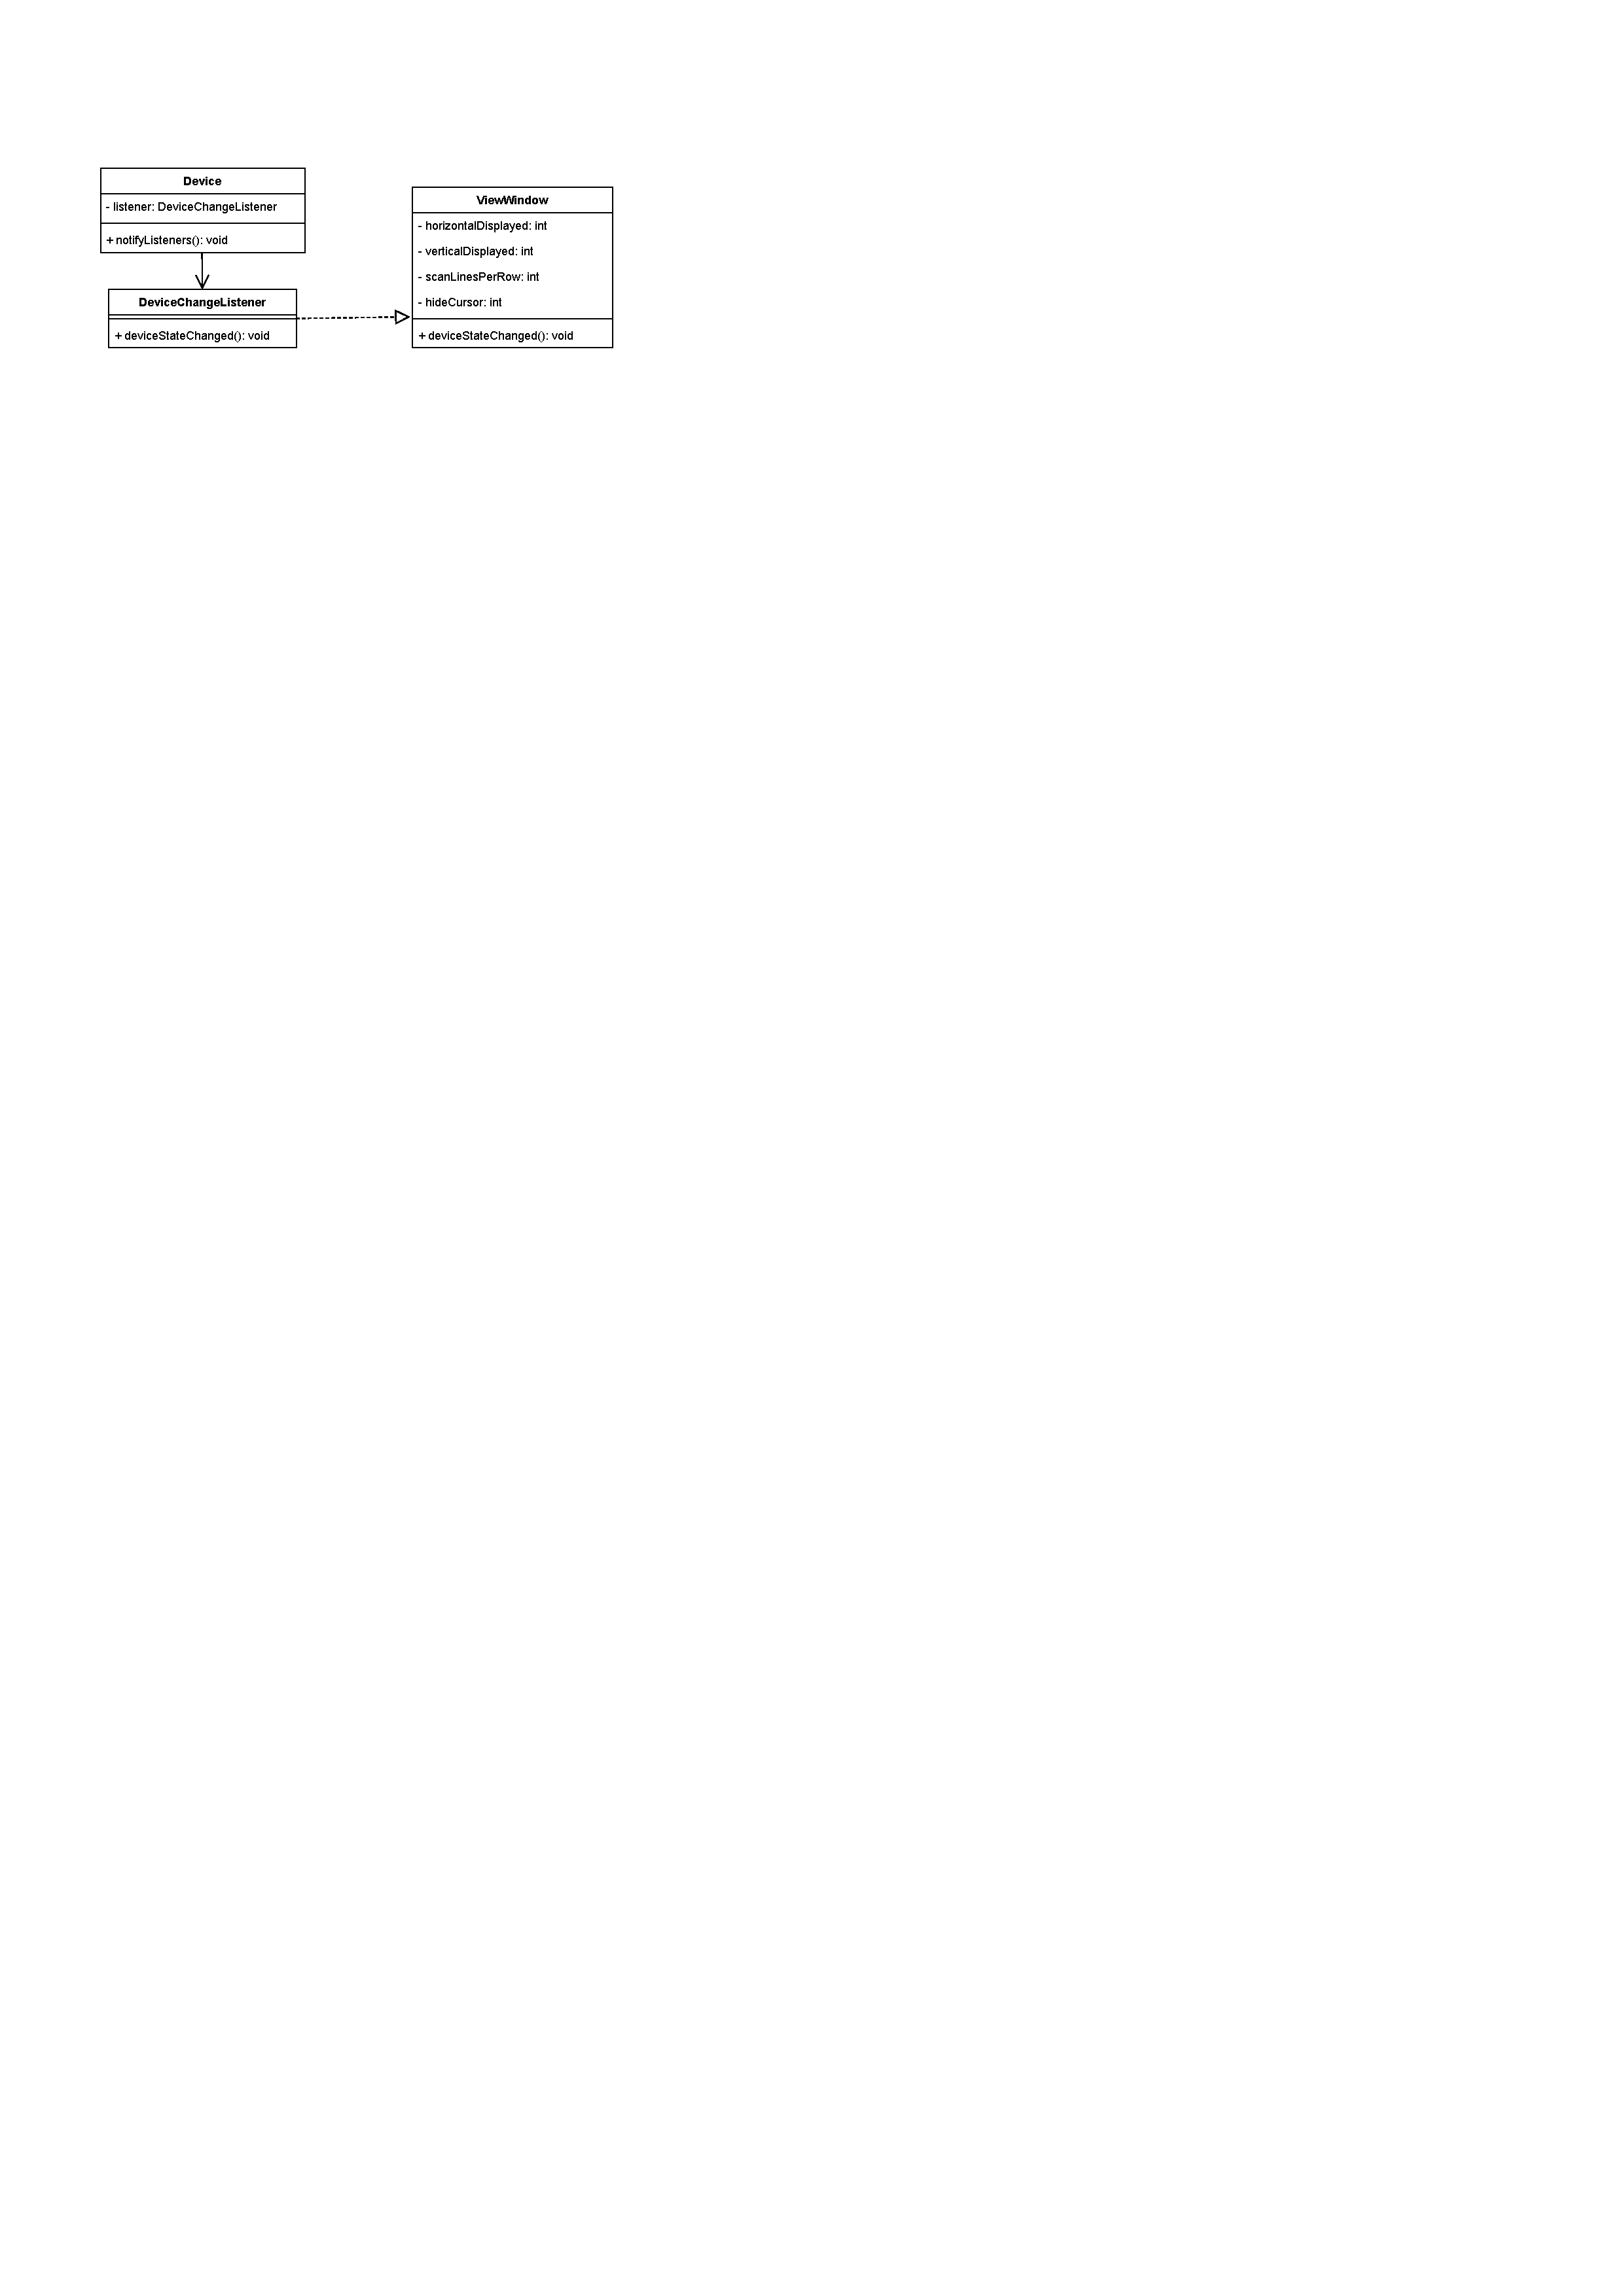
\includegraphics[width=0.9\textwidth]{figures/Observer.pdf}
  \caption{观察者模式在 Slow6502 中的类图}
\end{figure}


我们在 \lstinline{Device} 类里面使用了观察者模式,它有一个\lstinline{deviceChangeListeners}数组成员,可以通过\lstinline{notifyListener}函数以此调用它们的\lstinline{deviceStateChanged}函数,\lstinline{VideoWindow}实现了这个函数,会依次修改相应的属性。这样,当\lstinline{Device}类的状态发生变化时,它就可以通过调用观察者列表中的回调函数来通知观察者。

使用观察者模式的好处在于它可以让主体和观察者之间松散耦合。因为观察者只需要实现特定的回调函数,而主体只需要维护一个观察者列表,所以它们之间的依赖关系很少。这样,主体和观察者都可以独立地变化和扩展,而不会影响对方。